\documentclass[12pt]{article}
 
\usepackage[margin=1in]{geometry} 
\usepackage{amsmath,amsthm,amssymb}
\usepackage{hyperref}
\usepackage{graphicx}
\usepackage{xcolor}
\usepackage[many]{tcolorbox}
\tcbuselibrary{listings}
\usepackage{listings}

\usepackage{float}
\definecolor{lg}{HTML}{f0f0f0}

\newtcblisting{pycode}{
    colback=lg,
    boxrule=0pt,
    arc=0pt,
    outer arc=0pt,
    top=0pt,
    bottom=0pt,
    colframe=white,
    listing only,
    left=15.5pt,
    enhanced,
    listing options={
        basicstyle=\small\ttfamily,
        keywordstyle=\color{blue},
        language=Python,
        showstringspaces=false,
        tabsize=2,
        numbers=left,
        breaklines=true
    },
    overlay={
        \fill[gray!30]
        ([xshift=-3pt]frame.south west)
        rectangle
        ([xshift=11.5pt]frame.north west);
    }
}

\lstset{
    language=Python,
    basicstyle=\small\ttfamily,
}

 
\begin{document}
 
\title{Exercise 1}
\author{Cristian Manuel Abrante Dorta - 888248\\
ELEC-E8125 - Reinforcement Learning}

\maketitle
\section{Reward functions}
\label{sec:reward-functions}

\subsection{Task 1}
\label{sec:task-1}
\textbf {
    Train a model with 200 time steps per episode. Then test the model for 500 time steps.
}\\

For answering this question, first of all, the model had to be trained during 500 episodes with a maximum of 200 time steps per episode. After the agent is trained with those parameters a plot was generated in order to know the performance of the agent over the episodes:

\begin{figure}[ht]
    \centering
    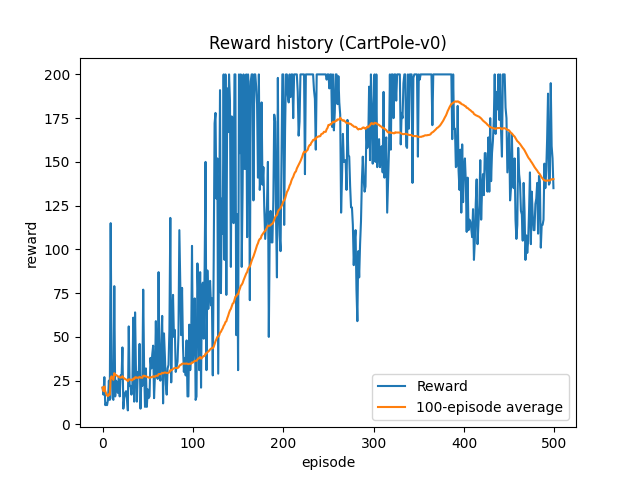
\includegraphics[scale=0.5]{exercise-1/report/img/task-1-training-200.png}
    \caption{Training result with 500 episodes and 200 max time steps per episode.}
    \label{fig:training-200}
\end{figure}

It is important to know that this is not a deterministic process, and that implies that the content of this plot is not the only possible training that the agent could have. But, as we can see in figure \ref{fig:training-200} the cumulative reward (equivalent to the maximum number of time steps that the pole was balanced), is increasing over the training episodes. Obtaining the maximum reward in some intervals between episodes 100 and 400. Also, the average reward has an increasing tendency over all the episodes except for the final 100 episodes. \\

After having trained the model, it was tested with a maximum of 500 timesteps per episode, and the obtained result was:

\begin{center}
    \texttt{Average test reward: 161.644 episode length: 161.644}
\end{center}

As we can see in this case, the agent did not generalized well, having an average test performance even worst than the parameter established for training which was 200 timesteps.

\subsection{Question 1.1}
\label{sec:question-1.1}
\textbf {
    Can the same model, trained to balance for 200 timesteps, also balance the pole for 500 timesteps? Briefily justify your answers.
}\\

The general answer to this question would be: yes it can. First of all, when the number of maximum time steps is increased, the main change is that the evaluation of the environment (in this case performed by \texttt{gym} using \texttt{env.step()}), is not going to consider the episode finalized (setting the \texttt{done} boolean variable to \texttt{true}) until the execution reaches 500 steps, or the pole falls.\\

So, as we previously trained the agent to balance the pole for 200 timesteps, theoretically it could continue doing it for more steps if it has generalized well during the training period. In practice, that is not happening in all the cases, mainly due to two reasons: On the one hand, the model is trained with 500 episodes, which could maybe not be enough for the generalization task, we can see that in Figure \ref{fig:training-200} where the variance between the average reward and some executions is really important. On the other hand, we have the maximum 200 train steps, which maybe is not enough too, we can see that also in the result of the test with 500 steps, which had as, a result, an average reward of 161.644. This result was even less than the 200 steps with which it was trained. 

\subsection{Task 2}
\label{sec:task-2}
\textbf {
    Repeat the experiment a few times, each time training the model from scratch with 200 time steps and testing it for 500 time steps.
}\\

The experiment was executed five different times from scratch, obtaining the corresponding training plots:

\begin{figure}[H]
   \begin{minipage}{0.32\textwidth}
     \centering
     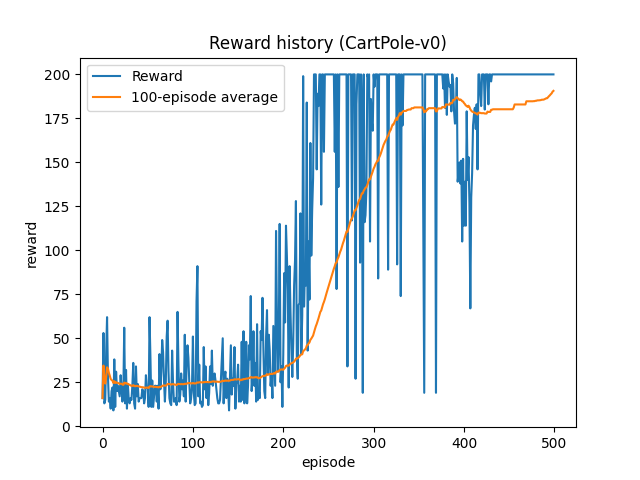
\includegraphics[width=\linewidth]{exercise-1/report/img/task-2-v1.png}
     \caption{First execution}
     \label{fig:task-2-v1}
   \end{minipage}\hfill
   \begin{minipage}{0.32\textwidth}
     \centering
     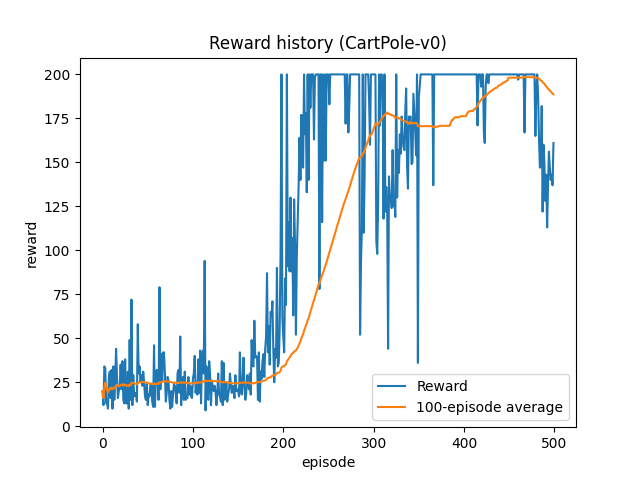
\includegraphics[width=\linewidth]{exercise-1/report/img/task-2-v2.png}
     \caption{Second execution}
     \label{fig:task-2-v2}
   \end{minipage}
   \begin{minipage}{0.32\textwidth}
     \centering
     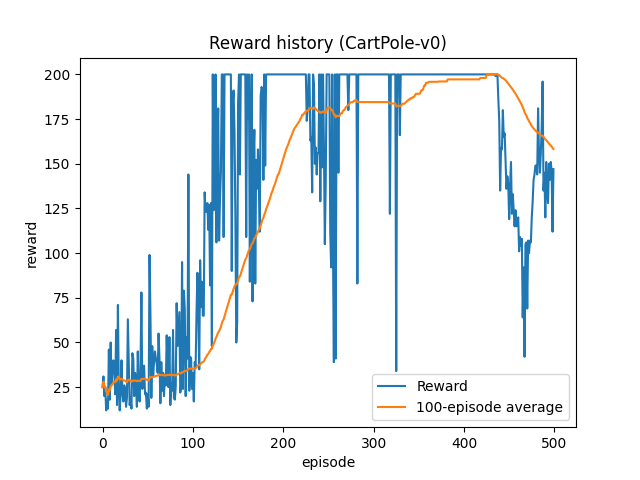
\includegraphics[width=\linewidth]{exercise-1/report/img/task-2-v3.png}
     \caption{Third execution}
     \label{fig:task-2-v3}
   \end{minipage}
\end{figure}

\begin{figure}[ht]
    \centering
   \begin{minipage}{0.48\textwidth}
     \centering
     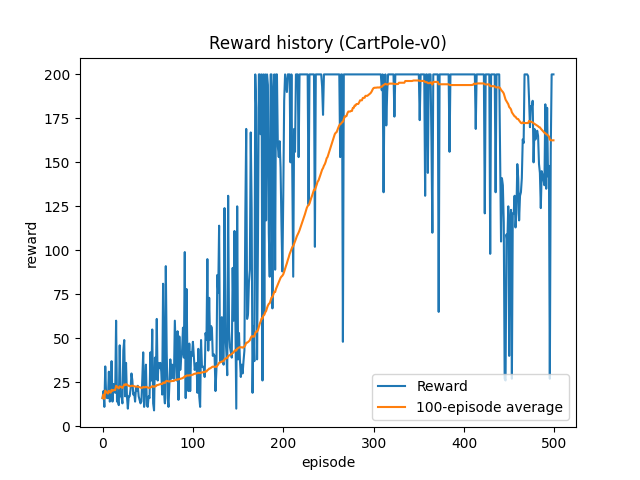
\includegraphics[width=0.68\linewidth]{exercise-1/report/img/task-2-v4.png}
     \caption{Fourth execution}
     \label{fig:task-2-v4}
   \end{minipage}\hfill
   \begin{minipage}{0.48\textwidth}
     \centering
     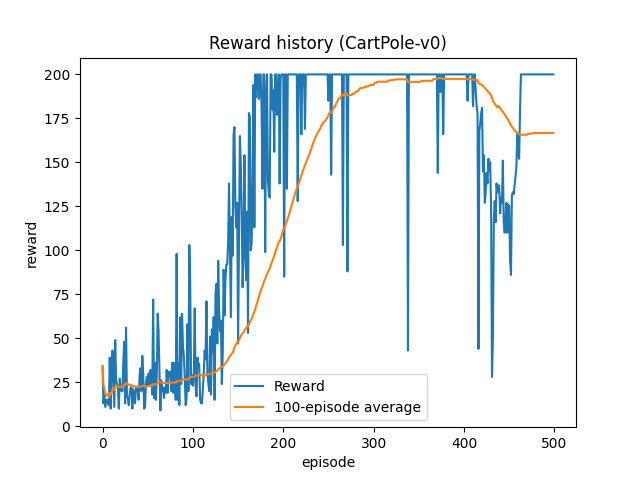
\includegraphics[width=0.68\linewidth]{exercise-1/report/img/task-2-v5.png}
     \caption{Fifth execution}
     \label{fig:task-2-v5}
   \end{minipage}
\end{figure}


Apart from the training plots, in the test phase, using 500 timesteps, we have obtained the following results stated in Table \ref{ref:rewards-table}.

\begin{table}[h]
\centering
\begin{tabular}{l|ccc}

\multicolumn{1}{l|}{Execution} & Figure                                      & \multicolumn{1}{l}{Average test reward} & \multicolumn{1}{l}{Episode length} \\ \hline
1                               & Figure \ref{fig:task-2-v1} & 497.632                                  & 497.632                             \\
2                               & Figure \ref{fig:task-2-v2} & 181.372                                  & 181.372                             \\
3                               & Figure \ref{fig:task-2-v3} & 138.476                                  & 138.476                             \\
4                               & Figure \ref{fig:task-2-v4} & 236.846                                  & 236.846                             \\
5                               & Figure \ref{fig:task-2-v5} & 299.016                                  & 299.016                            
\end{tabular}
\caption{Obtained rewards for the different executions}
\label{ref:rewards-table}
\end{table}

\subsection{Question 1.2}
\label{sec:question-1.2}
\textbf {
    Are the behavior and performance of the trained model the same every time? Analyze the causes briefly
}\\

As it was described in the previous section \ref{sec:question-1.1}, the system could achieve a better result than the 200 reward points that it was trained with, proof of that is the first execution, which achieved an average test reward of 497.632, which is almost the best possible reward that can be obtained. Apart from this execution, there have been others which has surpassed the barrier of the 200 reward points, such as the fifth and the sixth execution. 

It is remarkable to say that the behavior of the agent is not deterministic in any sense because the initial state is random each time the environment is initialized (when the episode ends), so the training has a different evolution each time that it is executed. The same happens with the test phase, that it is almost the same as the training phase but without the update of the outcome of the agent. \\

If we evaluate the performance in the graphic mode, we can do different observations. First of all, the trained agent learns to balance the pole even going to one side or the other, and that depends on the execution. Then, we can also observe that the agent learns to take advantage of the time and move from the border of the screen to finalize the episode in the established maximum time, in order to maximize the reward. Another relevant aspect is that the agent always follows a predefined direction (either goes left or right) and never changes the direction, even though this change could lead to more promising results (Figure \ref{fig:task-2-left} and Figure \ref{fig:task-2-right}).

\begin{figure}[ht]
    \centering
   \begin{minipage}{0.48\textwidth}
     \centering
     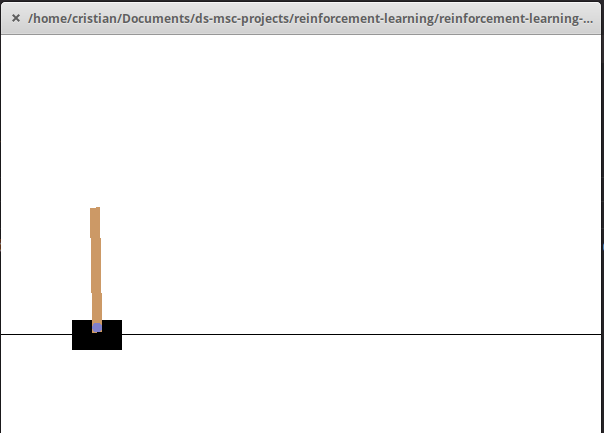
\includegraphics[width=0.7\linewidth]{exercise-1/report/img/task-2-left.png}
     \caption{Execution where the agent balanced the pole going to the left.}
     \label{fig:task-2-left}
   \end{minipage}\hfill
   \begin{minipage}{0.48\textwidth}
     \centering
     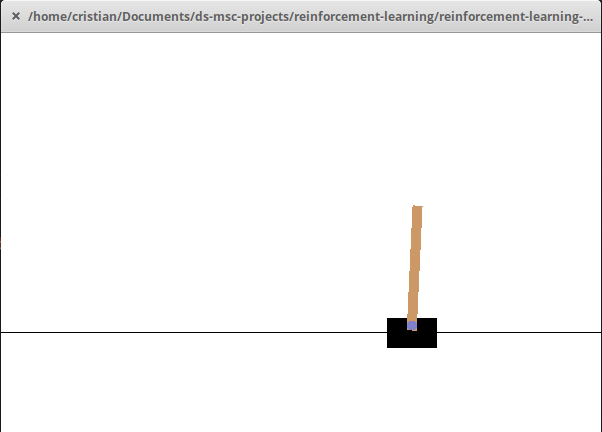
\includegraphics[width=0.7\linewidth]{exercise-1/report/img/task-2-right.png}
     \caption{Execution where the agent balanced the pole going to the right.}
     \label{fig:task-2-right}
   \end{minipage}
\end{figure}


\section{Task 2}
To embed code snippets in the report, you can use the \texttt{pycode} environment.

\begin{pycode}
for episode_number in range(train_episodes):
    reward_sum, timesteps = 0, 0
    done = False
    # Reset the environment and observe the initial state
    observation = env.reset()

    # Loop until the episode is over
    while not done:
        # Get action from the agent
        action, action_probabilities = agent.get_action(observation)
        previous_observation = observation

        # Perform the action on the environment, get new state and reward
        observation, reward, done, info = env.step(action)

        # Store action's outcome (so that the agent can improve its policy)
        agent.store_outcome(previous_observation, action_probabilities, action, reward)

        # Draw the frame, if desired
        if render:
            env.render()
\end{pycode}

\section{Question 1}

If you add a figure, you can refer to it using Figure.~\ref*{fig:fig1}.

\begin{figure}[h] 
	\centering  % Remember to centre the figure
    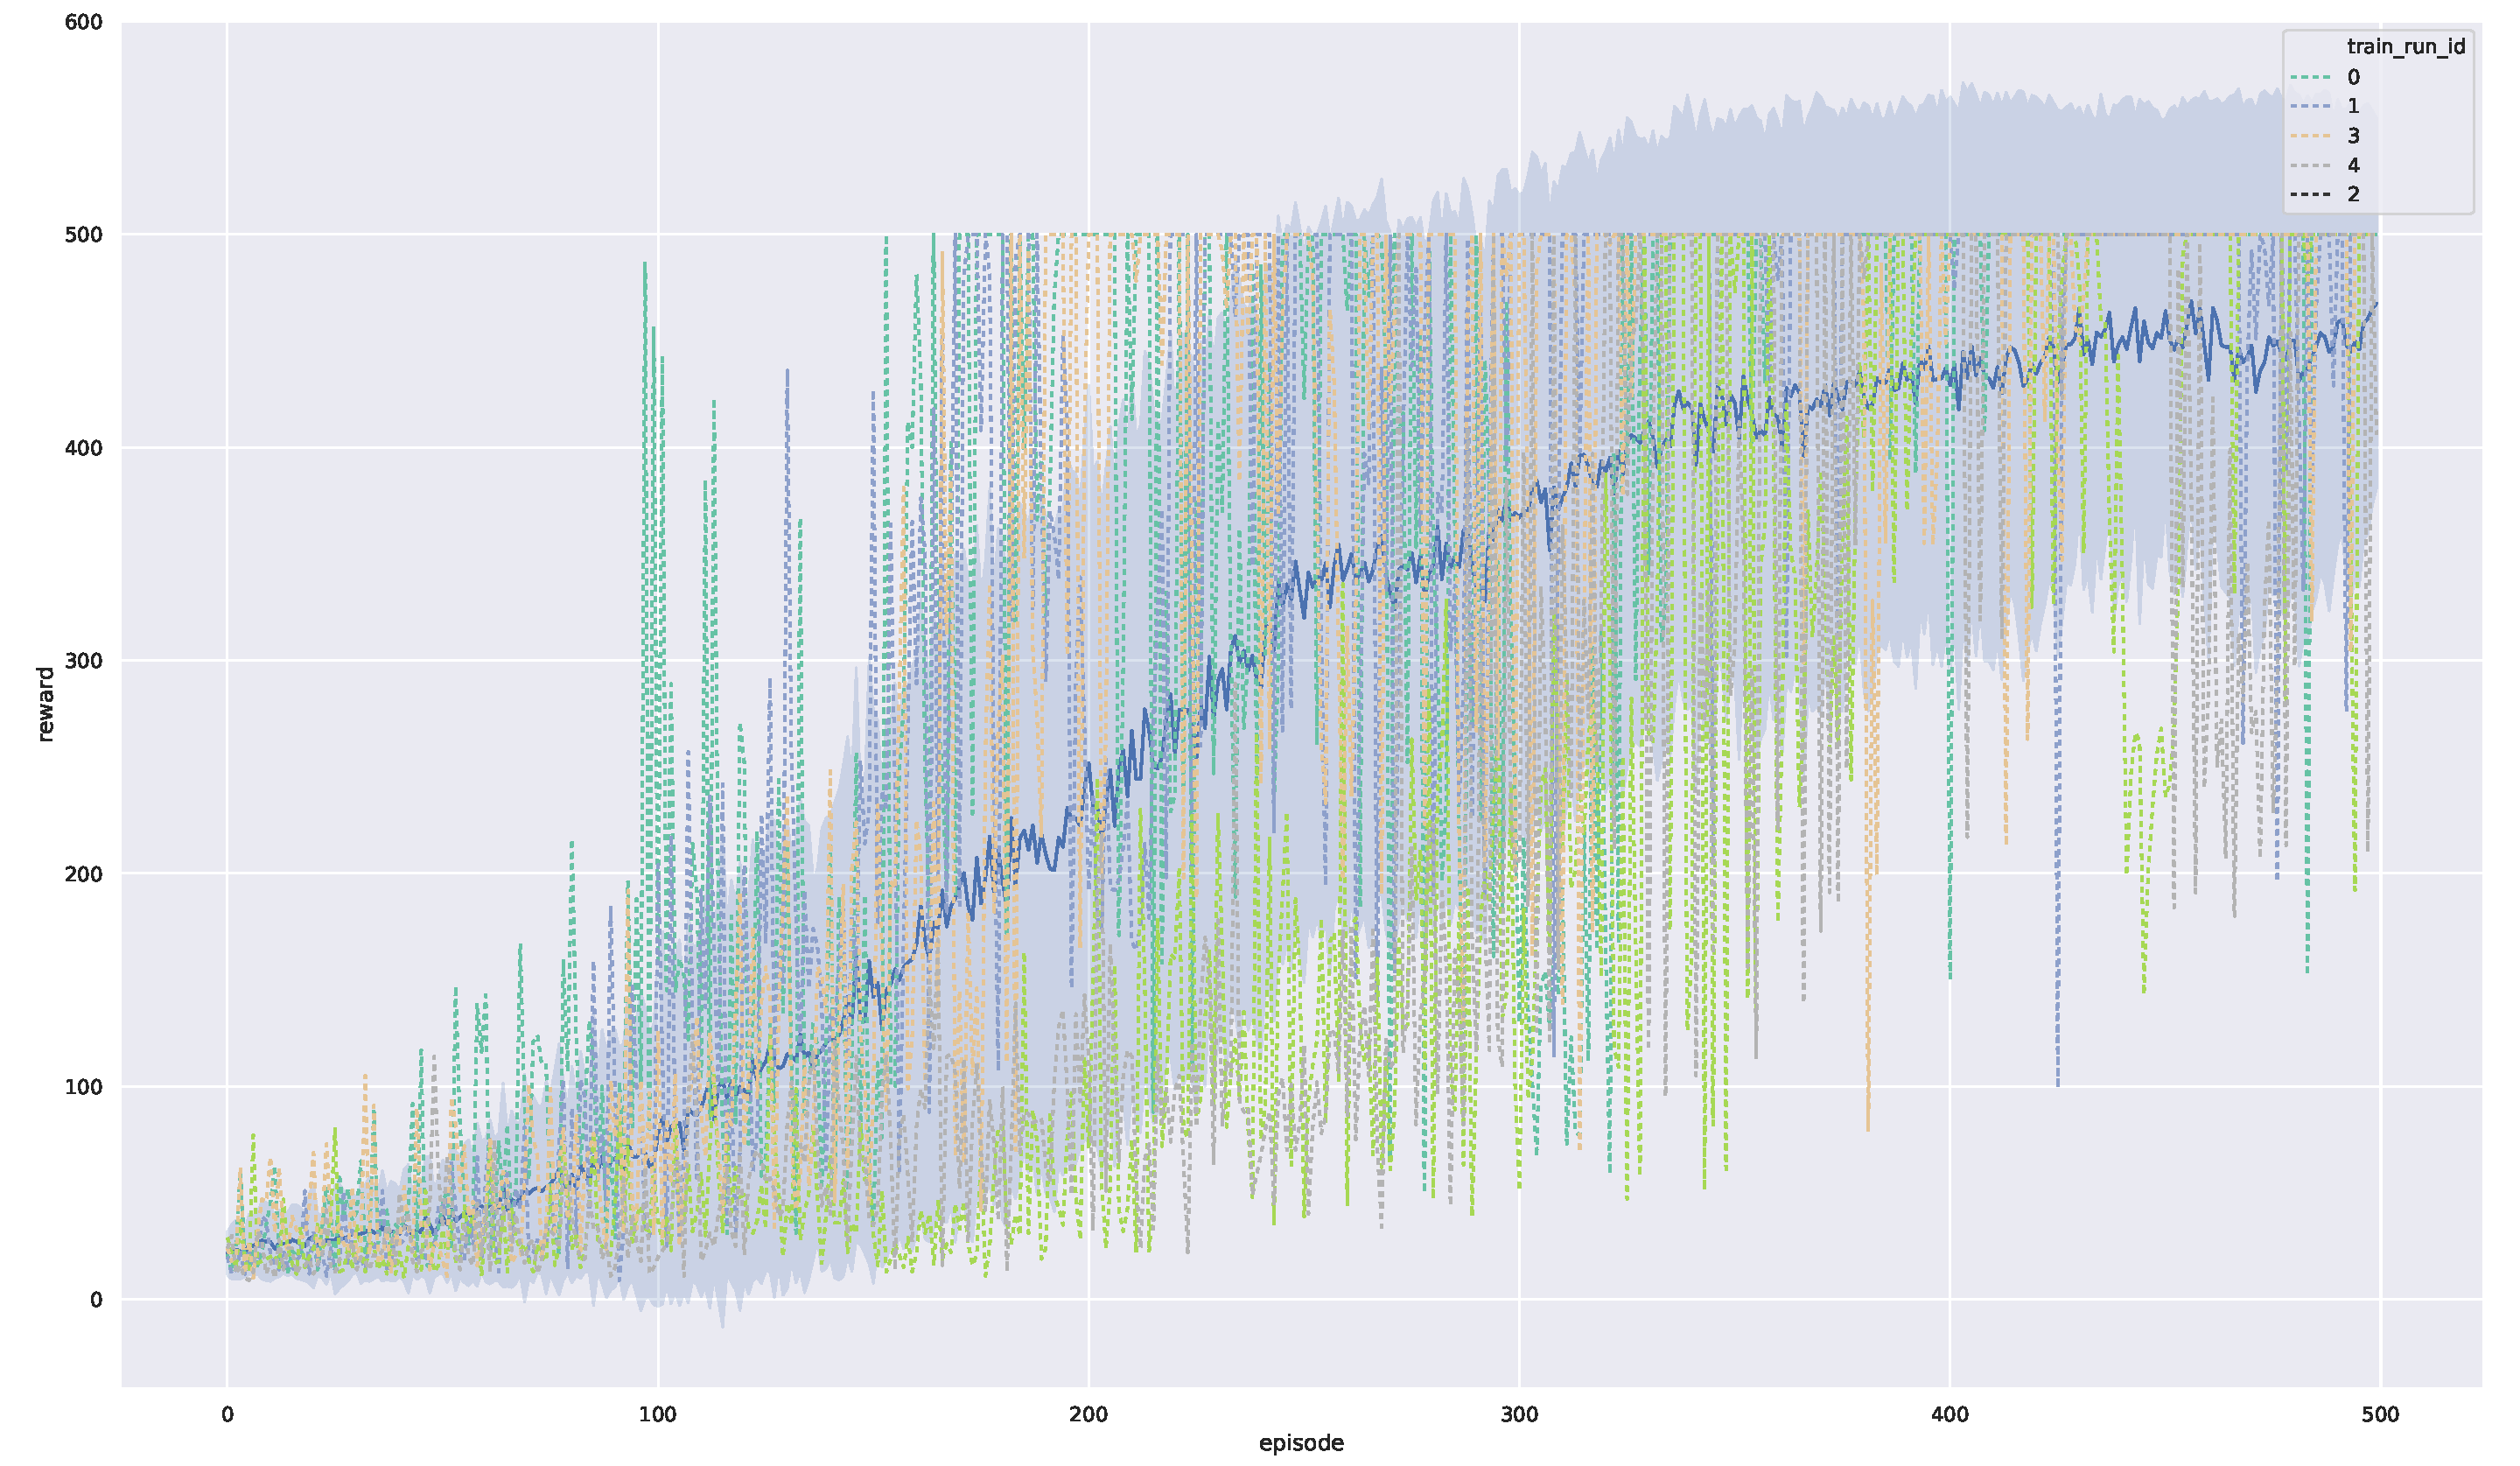
\includegraphics[width=0.9\columnwidth]{img/training.pdf}
	\caption{This is a sample figure.}
	\label{fig:fig1}
\end{figure}

\bibliographystyle{ieeetr}
\bibliography{template}  % Modify template with your bibliography name
\end{document}
